% ============================================================================
% MedivioAI — B.Tech Final Year Project Report
% AI-Powered Respiratory Disease Detection Platform
% Author: Aniket Ghosh
% ============================================================================

\documentclass[12pt, a4paper, oneside]{report}

% ======================== PACKAGES ========================
\usepackage[top=1in, bottom=1in, left=1.5in, right=1in]{geometry}
\usepackage{times}                    % Times New Roman
\usepackage{setspace}                 % Line spacing
\usepackage{graphicx}                 % Figures
\usepackage{float}                    % Figure placement
\usepackage{caption}                  % Captions
\usepackage{subcaption}               % Subfigures
\usepackage{booktabs}                 % Professional tables
\usepackage{longtable}                % Multi-page tables
\usepackage{array}                    % Table column types
\usepackage{tabularx}                 % Auto-width tables
\usepackage{multirow}                 % Multi-row cells
\usepackage{amsmath}                  % Equations
\usepackage{amssymb}                  % Math symbols
\usepackage{listings}                 % Code listings
\usepackage{xcolor}                   % Colors
\usepackage{hyperref}                 % Hyperlinks
\usepackage{url}                      % URL formatting
\usepackage{fancyhdr}                 % Headers/Footers
\usepackage{titlesec}                 % Section formatting
\usepackage{tocloft}                  % TOC formatting
\usepackage{nomencl}                  % Nomenclature
\usepackage{enumitem}                 % List formatting
\usepackage{pdfpages}                 % Include PDFs
\usepackage[utf8]{inputenc}           % UTF-8 encoding

% ======================== PAGE BORDER ========================
\usepackage{tikz}
\usepackage{eso-pic}
\AddToShipoutPictureBG{%
  \begin{tikzpicture}[remember picture, overlay]
    \draw[line width=1.5pt]
      ([xshift=0.75in, yshift=-0.5in]current page.north west)
      rectangle
      ([xshift=-0.5in, yshift=0.5in]current page.south east);
    \draw[line width=0.5pt]
      ([xshift=0.8in, yshift=-0.55in]current page.north west)
      rectangle
      ([xshift=-0.55in, yshift=0.55in]current page.south east);
  \end{tikzpicture}
}

% ======================== HYPERLINK SETUP ========================
\hypersetup{
    colorlinks=true,
    linkcolor=black,
    citecolor=blue,
    urlcolor=blue,
    bookmarksopen=true,
    pdfauthor={Aniket Ghosh},
    pdftitle={MedivioAI - AI-Powered Respiratory Disease Detection Platform},
}

% ======================== CODE LISTING STYLE ========================
\definecolor{codegreen}{rgb}{0,0.6,0}
\definecolor{codegray}{rgb}{0.5,0.5,0.5}
\definecolor{codepurple}{rgb}{0.58,0,0.82}
\definecolor{backcolour}{rgb}{0.97,0.97,0.97}

\lstdefinestyle{codestyle}{
    backgroundcolor=\color{backcolour},
    commentstyle=\color{codegreen},
    keywordstyle=\color{blue}\bfseries,
    numberstyle=\tiny\color{codegray},
    stringstyle=\color{codepurple},
    basicstyle=\ttfamily\small,
    breakatwhitespace=false,
    breaklines=true,
    captionpos=b,
    keepspaces=true,
    numbers=left,
    numbersep=5pt,
    showspaces=false,
    showstringspaces=false,
    showtabs=false,
    tabsize=2,
    frame=single,
    framerule=0.5pt,
    rulecolor=\color{codegray},
}
\lstset{style=codestyle}

% ======================== HEADER / FOOTER ========================
\pagestyle{fancy}
\fancyhf{}
\fancyfoot[C]{\thepage}
\renewcommand{\headrulewidth}{0pt}
\renewcommand{\footrulewidth}{0pt}

% ======================== SPACING ========================
\onehalfspacing

% ======================== PARAGRAPH FORMATTING ========================
\setlength{\parindent}{0pt}
\setlength{\parskip}{6pt}
\raggedright

% ======================== TITLE FORMATTING ========================
\titleformat{\chapter}[display]
  {\normalfont\Large\bfseries\centering}
  {\MakeUppercase{\chaptertitlename}\ \thechapter}{14pt}{\Large\MakeUppercase}
\titlespacing*{\chapter}{0pt}{-20pt}{20pt}

% ============================================================================
% DOCUMENT BEGINS
% ============================================================================
\begin{document}

% ======================== PRELIMINARY PAGES (Roman Numerals) ========================
\pagenumbering{roman}

% ======================== ABSTRACT ========================
\newpage
\addcontentsline{toc}{chapter}{Abstract}
\begin{center}
{\Large \textbf{ABSTRACT}}\\[1cm]
\end{center}

\singlespacing

Respiratory diseases, particularly Pneumonia and Tuberculosis, continue to be leading causes of morbidity and mortality worldwide, especially in resource-constrained healthcare settings where access to experienced radiologists remains limited. Timely and accurate analysis of Chest X-ray (CXR) images is critical for early intervention, yet manual interpretation is inherently subjective, time-intensive, and prone to diagnostic error under high patient volumes.

This project presents \textbf{MedivioAI}, an intelligent, full-stack web application designed to assist medical practitioners and radiologists in the early detection and screening of Pneumonia and Tuberculosis from standard posteroanterior Chest X-ray images. The system employs two dedicated Convolutional Neural Network (CNN) models: a \textbf{MobileNetV2}-based architecture for Pneumonia classification and a \textbf{DenseNet121}-based architecture for Tuberculosis detection. Both models are trained using transfer learning with ImageNet-pretrained weights and a two-phase training strategy comprising an initial frozen-base phase followed by selective fine-tuning of deeper layers to maximise feature extraction from medical radiographs.

The platform architecture follows a decoupled, three-tier microservice design. The \textbf{frontend}, built with React 19, Vite, and TailwindCSS, provides a responsive single-page application served globally via Vercel's edge network. The \textbf{backend API gateway}, implemented in Python Flask, manages user authentication via JSON Web Tokens (JWT) with bcrypt password hashing, handles image upload routing, and persists diagnostic records in a \textbf{MongoDB Atlas} cloud database. The memory-intensive TensorFlow inference workloads are offloaded to a dedicated \textbf{Hugging Face Spaces} Docker container provisioned with 16\,GB of RAM, thereby decoupling compute-heavy model serving from the lightweight API tier and enabling the entire platform to operate within free-tier hosting constraints.

The Tuberculosis detection model achieved a test accuracy of \textbf{98.89\%}, precision of \textbf{98.04\%}, recall of \textbf{95.24\%}, F1-score of \textbf{96.62\%}, and an AUC-ROC of \textbf{0.9985} on 630 test samples. The system processes a complete prediction cycle---from image upload through inference to result display---in under three seconds. Additional features include a patient medical history dashboard, PDF report generation using jsPDF, image thumbnail persistence, and a searchable diagnostic record log.

\vspace{0.5cm}
\noindent\textbf{Keywords:} Deep Learning, Convolutional Neural Networks, Transfer Learning, Pneumonia Detection, Tuberculosis Detection, Chest X-ray Analysis, MobileNetV2, DenseNet121, Flask, React, MongoDB, Microservice Architecture, Medical Image Classification.

\onehalfspacing

% ======================== TABLE OF CONTENTS ========================
\newpage
\tableofcontents

% ======================== LIST OF TABLES ========================
\newpage
\addcontentsline{toc}{chapter}{List of Tables}
\listoftables

% ======================== LIST OF FIGURES ========================
\newpage
\addcontentsline{toc}{chapter}{List of Figures}
\listoffigures

% ======================== LIST OF ABBREVIATIONS ========================
\newpage
\addcontentsline{toc}{chapter}{List of Abbreviations}
\begin{center}
{\Large \textbf{LIST OF ABBREVIATIONS}}\\[1cm]
\end{center}

\begin{longtable}{p{3.5cm} p{10cm}}
\toprule
\textbf{Abbreviation} & \textbf{Full Form} \\
\midrule
\endfirsthead
\toprule
\textbf{Abbreviation} & \textbf{Full Form} \\
\midrule
\endhead

AI & Artificial Intelligence \\
API & Application Programming Interface \\
AUC & Area Under the Curve \\
CNN & Convolutional Neural Network \\
CORS & Cross-Origin Resource Sharing \\
CPU & Central Processing Unit \\
CXR & Chest X-Ray \\
DL & Deep Learning \\
ER & Entity-Relationship \\
GPU & Graphics Processing Unit \\
HF & Hugging Face \\
HTTPS & HyperText Transfer Protocol Secure \\
JSON & JavaScript Object Notation \\
JWT & JSON Web Token \\
ML & Machine Learning \\
MCC & Matthews Correlation Coefficient \\
NoSQL & Not Only Structured Query Language \\
PDF & Portable Document Format \\
RAM & Random Access Memory \\
REST & Representational State Transfer \\
RGB & Red, Green, Blue \\
ROC & Receiver Operating Characteristic \\
SPA & Single Page Application \\
TB & Tuberculosis \\
UI & User Interface \\
UML & Unified Modeling Language \\
UX & User Experience \\
WHO & World Health Organisation \\
\bottomrule
\end{longtable}

% ======================== CHAPTERS (Arabic Numerals) ========================
\newpage
\pagenumbering{arabic}

% ============================================================================
% CHAPTER 1: INTRODUCTION
% ============================================================================
\chapter{Introduction}
\label{chap:introduction}

\section{Background}
\label{sec:background}

Respiratory diseases represent a significant global health burden. According to the World Health Organisation (WHO), Pneumonia remains the single largest infectious cause of death in children worldwide, accounting for approximately 14\% of all deaths of children under five years of age. Tuberculosis (TB), caused by \textit{Mycobacterium tuberculosis}, infected an estimated 10.6 million people in 2022, with 1.3 million deaths reported globally. In developing nations, the shortage of trained radiologists exacerbates the diagnostic bottleneck: chest radiographs (X-rays) remain the most widely available and cost-effective imaging modality for pulmonary screening, yet their interpretation requires considerable expertise and is subject to inter-observer variability.

The convergence of deep learning and medical imaging has opened new avenues for computer-aided diagnosis (CAD) systems. Convolutional Neural Networks (CNNs), in particular, have demonstrated near-expert-level performance in classifying medical images across a range of pathologies. Transfer learning---the practice of initialising a neural network with weights pre-trained on large-scale general-purpose datasets such as ImageNet---has further reduced the data requirements and training time for domain-specific medical imaging tasks. These advances make it feasible to deploy AI-assisted diagnostic tools even in settings with limited computational resources and labelled data.

\section{Motivation}
\label{sec:motivation}

The primary motivation for developing MedivioAI arises from three intersecting challenges observed in current clinical workflows:

\begin{enumerate}[label=\arabic*.]
    \item \textbf{Diagnostic Delay:} In many primary healthcare centres, chest X-ray films are collected locally but must be transported to a distant radiology centre for interpretation, introducing delays of hours to days. An AI-assisted screening tool that provides instant probabilistic feedback directly at the point of care can facilitate faster triage and earlier treatment initiation.

    \item \textbf{Scalability of Expertise:} Training a radiologist requires years of specialised education. A software system that encodes learned diagnostic patterns from thousands of labelled radiographs can serve as a force multiplier, extending the effective reach of scarce specialist expertise to underserved regions.

    \item \textbf{Cost-Effective Deployment:} Most existing medical AI solutions require dedicated GPU servers or expensive cloud inference APIs. MedivioAI demonstrates that a production-grade diagnostic platform can be architected using exclusively free-tier cloud services---Vercel for the frontend, Render for the API gateway, Hugging Face Spaces for model inference, and MongoDB Atlas for data persistence---without compromising prediction latency or user experience.
\end{enumerate}

\section{Objectives}
\label{sec:objectives}

The specific objectives of this project are as follows:

\begin{enumerate}[label=\arabic*.]
    \item To design and train two dedicated CNN classifiers---one for Pneumonia detection (using MobileNetV2 as the base architecture) and one for Tuberculosis detection (using DenseNet121)---employing transfer learning and a two-phase training strategy.

    \item To develop a responsive, modern web-based user interface using React 19 and TailwindCSS that allows medical practitioners to upload Chest X-ray images and receive real-time diagnostic predictions with probability scores.

    \item To implement a secure RESTful API backend using Python Flask, incorporating JWT-based authentication, bcrypt password hashing, and MongoDB Atlas for persistent user account and medical record management.

    \item To architect a decoupled microservice deployment pipeline that offloads compute-intensive model inference to Hugging Face Spaces (Docker), thereby operating the entire platform within free-tier hosting constraints.

    \item To provide auxiliary features including a patient dashboard with diagnostic history, searchable records with image thumbnails, and downloadable PDF diagnostic reports.
\end{enumerate}

\section{Scope of the Project}
\label{sec:scope}

MedivioAI is scoped as an \textit{experimental AI-assisted screening tool} and is not intended to serve as a stand-alone diagnostic device or a replacement for professional radiological assessment. The system is designed for posteroanterior (PA) Chest X-ray images and classifies each image into one of two classes per model: \textit{Normal} versus \textit{Pneumonia}, or \textit{Normal} versus \textit{Tuberculosis}. Multi-label classification (simultaneous detection of multiple pathologies) and advanced interpretability features such as Gradient-weighted Class Activation Mapping (Grad-CAM) are identified as future enhancements and fall outside the current scope.

\section{Organisation of the Report}
\label{sec:organisation}

The remainder of this report is organised as follows:

\begin{itemize}
    \item \textbf{Chapter 2} presents a comprehensive literature survey covering prior work in medical image classification, transfer learning strategies, and existing CAD systems for respiratory disease detection.
    \item \textbf{Chapter 3} formally defines the problem statement and describes the system modules and their functionalities.
    \item \textbf{Chapter 4} details the software design, including system architecture diagrams, data flow diagrams, UML component and sequence diagrams, and the entity-relationship model.
    \item \textbf{Chapter 5} specifies the software and hardware requirements for development and deployment.
    \item \textbf{Chapter 6} presents the code architecture, explaining each module with its classes, methods, input parameters, output values, and database schema.
    \item \textbf{Chapter 7} showcases the output screens, user interfaces, and experimental results including model performance metrics and evaluation plots.
    \item \textbf{Chapter 8} provides the conclusions, summarises the contributions, and outlines directions for future work.
\end{itemize}

% ============================================================================
% CHAPTER 2: LITERATURE SURVEY
% ============================================================================
\chapter{Literature Survey}
\label{chap:literature}

\section{Medical Image Classification Using Deep Learning}
\label{sec:medical_image_dl}

The application of deep learning to medical image analysis has grown rapidly since the landmark demonstration by Krizhevsky et al. (2012) that deep convolutional neural networks could significantly outperform traditional hand-crafted feature extractors on the ImageNet Large Scale Visual Recognition Challenge~[1]. Subsequent architectures---VGGNet~[2], GoogLeNet~[3], ResNet~[4], DenseNet~[5], and the MobileNet family~[6]---progressively improved classification accuracy while also exploring model efficiency for deployment on resource-constrained devices.

In the medical domain, Rajpurkar et al. (2017) introduced CheXNet, a 121-layer DenseNet trained on the ChestX-ray14 dataset comprising over 100{,}000 frontal-view chest radiographs~[7]. CheXNet achieved an F1 score that exceeded the average performance of four practising radiologists on the Pneumonia detection task, demonstrating that deep CNNs can reach or surpass human-level performance on specific diagnostic subtasks.

\section{Transfer Learning in Medical Imaging}
\label{sec:transfer_learning}

Transfer learning addresses the fundamental challenge of limited labelled data in medical imaging by leveraging representations learned from large-scale general-purpose datasets. Yosinski et al. (2014) showed that early convolutional layers learn generic features (edges, textures, colour gradients) that are transferable across tasks, while deeper layers learn increasingly task-specific features~[8]. In the medical imaging context, Shin et al. (2016) demonstrated that fine-tuning ImageNet-pretrained CNNs consistently outperforms training from scratch, even when the target domain (medical radiographs) differs substantially from the source domain (natural photographs)~[9].

The two-phase training strategy adopted in MedivioAI---initial training with frozen base layers followed by selective fine-tuning of deeper layers with a reduced learning rate---is a well-established practice that prevents catastrophic forgetting of learned general features while allowing the network to adapt to the specific statistical characteristics of medical X-ray images~[10].

\section{Pneumonia Detection from Chest X-Rays}
\label{sec:pneumonia_literature}

Kermany et al. (2018) curated a benchmark dataset of 5{,}856 validated chest X-ray images categorised into Pneumonia and Normal classes, which has since become one of the most widely used datasets for pneumonia classification research~[11]. Their work employed transfer learning with Inception V3 and achieved a classification accuracy of approximately 92.8\%. Subsequent studies have reported improved results using architectures such as ResNet-50 (accuracy $\sim$95\%), VGG-16 (accuracy $\sim$93\%), and MobileNetV2 (accuracy $\sim$94\%), the latter being particularly attractive for deployment scenarios due to its significantly smaller model size and inference time~[12].

MobileNetV2, proposed by Sandler et al. (2018), introduces inverted residual blocks with linear bottlenecks that achieve competitive accuracy with a model size approximately 14$\times$ smaller than VGG-16~[6]. This architectural efficiency makes MobileNetV2 an ideal choice for the Pneumonia detection model in MedivioAI, where inference is performed on a cloud container with finite memory resources.

\section{Tuberculosis Detection from Chest X-Rays}
\label{sec:tb_literature}

Automated TB screening from chest X-rays has been explored using both traditional machine learning pipelines (using hand-crafted features such as Gabor filters, local binary patterns, and histogram of oriented gradients) and deep learning approaches. Lakhani and Sundaram (2017) demonstrated that an ensemble of AlexNet and GoogLeNet achieved an AUC of 0.99 on a curated TB dataset~[13]. Hwang et al. (2016) developed a CAD system based on a deep CNN that performed comparably to radiologists in a multi-reader study~[14].

DenseNet121, proposed by Huang et al. (2017), connects each layer to every other layer in a feed-forward fashion, promoting feature reuse and substantially reducing the number of parameters compared to traditional architectures of similar depth~[5]. In the context of chest X-ray analysis, DenseNet121 has been the backbone of CheXNet and several subsequent systems, making it a well-validated choice for the Tuberculosis detection model in MedivioAI.

\section{Existing Computer-Aided Diagnosis Systems}
\label{sec:existing_cad}

Several commercial and research CAD systems have been developed for chest X-ray analysis:

\begin{itemize}
    \item \textbf{qXR (Qure.ai):} A WHO-recommended AI solution for TB screening that provides heatmap overlays and has been deployed in over 45 countries~[15].
    \item \textbf{Lunit INSIGHT CXR:} Detects 10 major chest X-ray findings using a deep learning model with a reported AUC above 0.98 for TB detection~[16].
    \item \textbf{CheXpert (Stanford ML Group):} A large-scale publicly available dataset and associated models for multi-label chest X-ray classification~[17].
\end{itemize}

While these systems demonstrate excellent diagnostic performance, they typically require dedicated GPU infrastructure, commercial licensing, or are limited to research use. MedivioAI distinguishes itself by providing a fully open-source, zero-cost deployment architecture that is accessible to educational institutions and resource-limited healthcare settings.

\section{Summary of Literature Review}
\label{sec:literature_summary}

Table~\ref{tab:literature_summary} summarises the key studies and their relevance to the present work.

\begin{table}[H]
\centering
\caption{Summary of literature review}
\label{tab:literature_summary}
\begin{tabularx}{\textwidth}{>{\raggedright\arraybackslash}p{3.5cm} >{\raggedright\arraybackslash}p{3cm} >{\raggedright\arraybackslash}p{3cm} >{\raggedright\arraybackslash}X}
\toprule
\textbf{Study} & \textbf{Architecture} & \textbf{Task} & \textbf{Key Finding} \\
\midrule
Rajpurkar et al. (2017) & DenseNet-121 & Pneumonia detection & Exceeded radiologist-level F1 score \\
Kermany et al. (2018) & Inception V3 & Pneumonia classification & 92.8\% accuracy on 5{,}856 CXR images \\
Sandler et al. (2018) & MobileNetV2 & General classification & 14$\times$ smaller than VGG-16 with competitive accuracy \\
Lakhani \& Sundaram (2017) & AlexNet + GoogLeNet & TB detection & AUC of 0.99 on TB dataset \\
Huang et al. (2017) & DenseNet-121 & Image classification & Feature reuse through dense connections \\
\bottomrule
\end{tabularx}
\end{table}

% ============================================================================
% CHAPTER 3: PROBLEM DEFINITION, MODULES AND FUNCTIONALITIES
% ============================================================================
\chapter{Definition of the Problem with Modules and Functionalities}
\label{chap:problem}

\section{Problem Statement}
\label{sec:problem_statement}

The central problem addressed by this project can be formally stated as follows: Given a posteroanterior (PA) Chest X-ray image $I$ of dimensions $H \times W \times C$, design and implement an end-to-end web-based system that (a)~preprocesses $I$ to a standardised tensor of shape $(224, 224, 3)$ with pixel values normalised to $[0, 1]$, (b)~passes the preprocessed tensor through a trained CNN classifier $f_\theta$ to produce a posterior probability $p = f_\theta(I) \in [0, 1]$, (c)~applies a decision threshold $\tau = 0.5$ such that the predicted class $\hat{y} = \begin{cases} \text{DISEASE} & \text{if } p > \tau \\ \text{NORMAL} & \text{if } p \leq \tau \end{cases}$, and (d)~returns $\hat{y}$ along with confidence scores to the user through a web interface within a response time of under three seconds.

\section{System Modules}
\label{sec:modules}

The MedivioAI platform is decomposed into the following distinct modules:

\subsection{Module 1: User Authentication and Account Management}
\label{subsec:mod_auth}

This module handles secure user registration, login, and session management. The key functionalities include:

\begin{itemize}
    \item \textbf{User Registration:} Accepts name, email, password, age (optional), and gender (optional). The password is hashed using the bcrypt algorithm with a randomly generated salt before storage. A unique index on the email field prevents duplicate accounts.
    \item \textbf{User Login:} Validates credentials against stored bcrypt hashes. Upon successful authentication, a JSON Web Token (JWT) is generated with a 7-day expiry, encoding the user's MongoDB ObjectId in the \texttt{sub} claim.
    \item \textbf{Profile Retrieval:} Returns the authenticated user's profile data by decoding the JWT from the \texttt{Authorization: Bearer <token>} header and fetching the corresponding document from the \texttt{users} collection.
    \item \textbf{Session Persistence:} The frontend persists the JWT in \texttt{localStorage} and the user object in \texttt{sessionStorage} to maintain state across page refreshes.
\end{itemize}

\subsection{Module 2: Image Upload and Preprocessing}
\label{subsec:mod_upload}

This module manages the intake of Chest X-ray images from the user's device. Functionalities include:

\begin{itemize}
    \item \textbf{Drag-and-Drop and File Picker:} The React \texttt{SinglePrediction} component supports both drag-and-drop and click-to-browse interactions for image selection.
    \item \textbf{Client-Side Validation:} Only files with MIME types beginning with \texttt{image/} are accepted. Supported formats include JPEG, JPG, and PNG with a maximum size of 10\,MB.
    \item \textbf{Image Preview:} Upon file selection, a \texttt{FileReader} generates a base64-encoded Data URL that is rendered as an inline preview.
    \item \textbf{Form Data Construction:} The selected file and model name (\texttt{pneumonia} or \texttt{tuberculosis}) are packaged into a \texttt{FormData} object for multipart upload to the backend.
\end{itemize}

\subsection{Module 3: AI Inference Engine}
\label{subsec:mod_inference}

The inference engine is the computational core of the system and operates as follows:

\begin{itemize}
    \item \textbf{Request Routing:} The Flask backend receives the uploaded image at the \texttt{/api/predict} endpoint and forwards the raw image bytes along with the model selector to the Hugging Face Space inference endpoint via an HTTPS POST request.
    \item \textbf{Image Preprocessing (Server-Side):} At the Hugging Face container, the image is resized to $224 \times 224$ pixels, converted to RGB colour space, and normalised by dividing pixel values by 255.0.
    \item \textbf{Model Inference:} The preprocessed tensor is fed to the appropriate Keras model (MobileNetV2 for Pneumonia or DenseNet121 for Tuberculosis). The sigmoid activation in the final layer outputs a scalar probability $p$.
    \item \textbf{Classification:} If $p > 0.5$, the system returns \texttt{PNEUMONIA} or \texttt{TUBERCULOSIS} with confidence $c = p \times 100\%$. Otherwise, it returns \texttt{NORMAL} with confidence $c = (1 - p) \times 100\%$.
\end{itemize}

\subsection{Module 4: Medical Records Management}
\label{subsec:mod_records}

If the user is authenticated (determined by optionally parsing the JWT from the request header), a diagnostic record is persisted in MongoDB. The record includes:

\begin{itemize}
    \item \texttt{user\_id}: MongoDB ObjectId linking the record to the user.
    \item \texttt{model\_used}: String indicating the model (\texttt{pneumonia} or \texttt{tuberculosis}).
    \item \texttt{prediction}: The classification result (\texttt{NORMAL}, \texttt{PNEUMONIA}, or \texttt{TUBERCULOSIS}).
    \item \texttt{confidence}: Rounded confidence percentage.
    \item \texttt{probability}: Object containing normalised probabilities for both classes.
    \item \texttt{timestamp}: UTC timestamp of the prediction.
    \item \texttt{filename}: Original filename of the uploaded image.
    \item \texttt{image\_preview}: A base64-encoded JPEG thumbnail (150$\times$150 pixels) of the uploaded X-ray.
\end{itemize}

\subsection{Module 5: Patient Dashboard and Reporting}
\label{subsec:mod_dashboard}

The dashboard module provides:

\begin{itemize}
    \item \textbf{Profile Display:} Shows the authenticated user's name, email, age, and gender.
    \item \textbf{Diagnosis History Table:} Lists all past scans in reverse chronological order with thumbnail previews, model type, prediction result, confidence percentage with visual progress bar, and date-time stamps.
    \item \textbf{Search and Filter:} A search bar allows filtering records by prediction result, model name, or filename.
    \item \textbf{PDF Report Generation:} Each record can be exported as a formatted PDF using the jsPDF library, including patient metadata, prediction details, a disclaimer, and an embedded image preview.
    \item \textbf{Refresh:} A manual refresh button re-fetches records from the backend.
\end{itemize}

\subsection{Module 6: Model Training and Evaluation Pipeline}
\label{subsec:mod_training}

Although model training is an offline activity, the pipeline scripts are integral to the project:

\begin{itemize}
    \item \textbf{Data Processing:} Scripts for scanning source directories, validating image integrity, splitting data into train/validation/test sets (70/15/15 ratio for TB), and copying files to a structured directory layout.
    \item \textbf{Model Training:} Two-phase training (frozen base, then selective fine-tuning) with callbacks for model checkpointing (best validation accuracy), early stopping (patience of 10 epochs), learning rate reduction on plateau, and CSV/TensorBoard logging.
    \item \textbf{Model Evaluation:} Generation of confusion matrices, ROC curves, precision-recall curves, classification reports, and aggregated metrics (accuracy, precision, recall, F1, AUC-ROC, MCC) saved as JSON and image artefacts.
\end{itemize}

% ============================================================================
% CHAPTER 4: SOFTWARE DESIGN
% ============================================================================
\chapter{Software Design}
\label{chap:design}

\section{System Architecture Diagram}
\label{sec:architecture}

The MedivioAI platform follows a three-tier microservice architecture, as illustrated in Fig.~\ref{fig:system_arch}. The three tiers are: (1)~the client-side React single-page application, (2)~the Flask API gateway, and (3)~the Hugging Face Spaces inference container. Each tier is independently deployed and communicates over HTTPS.

\begin{figure}[H]
\centering
\fbox{\parbox{0.9\textwidth}{\centering
\vspace{0.5cm}
\textbf{[System Architecture Diagram Placeholder]}\\[0.3cm]
\small
\texttt{Web Browser (React/Vite on Vercel)} $\xrightarrow{\text{HTTPS/JSON}}$
\texttt{Flask API Gateway (Render)} $\xrightarrow{\text{HTTPS/multipart}}$
\texttt{HF Space Docker (TensorFlow)}\\[0.2cm]
\texttt{Flask API Gateway} $\xleftrightarrow{\text{pymongo}}$ \texttt{MongoDB Atlas Cloud}
\vspace{0.5cm}
}}
\caption{Three-tier microservice architecture of MedivioAI}
\label{fig:system_arch}
\end{figure}

\textbf{Design Rationale:} The decision to separate the model inference container from the API gateway was driven by the memory constraints of Render's free tier (512\,MB RAM). Loading TensorFlow and the Keras models into memory would exceed this limit. By delegating inference to Hugging Face Spaces, which provides containers with 16\,GB RAM on the free tier, the system achieves reliable predictions without incurring hosting costs.

\section{Data Flow Diagram}
\label{sec:dfd}

\subsection{Level 0 DFD (Context Diagram)}

\begin{figure}[H]
\centering
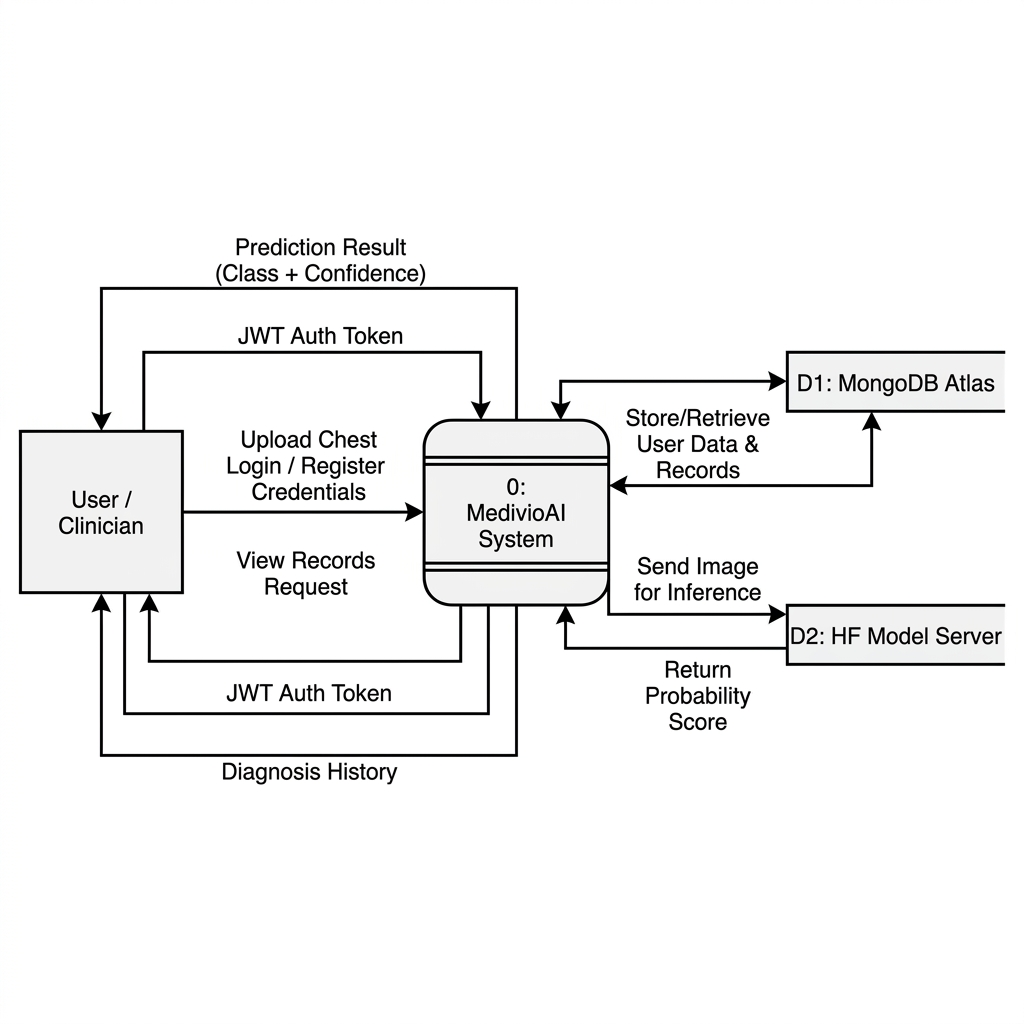
\includegraphics[width=0.9\textwidth]{dfd_level0.png}
\caption{Level 0 Data Flow Diagram (Context Diagram)}
\label{fig:dfd_level0}
\end{figure}

\subsection{Level 1 DFD}

The Level 1 DFD decomposes the system into six major processes:

\begin{figure}[H]
\centering
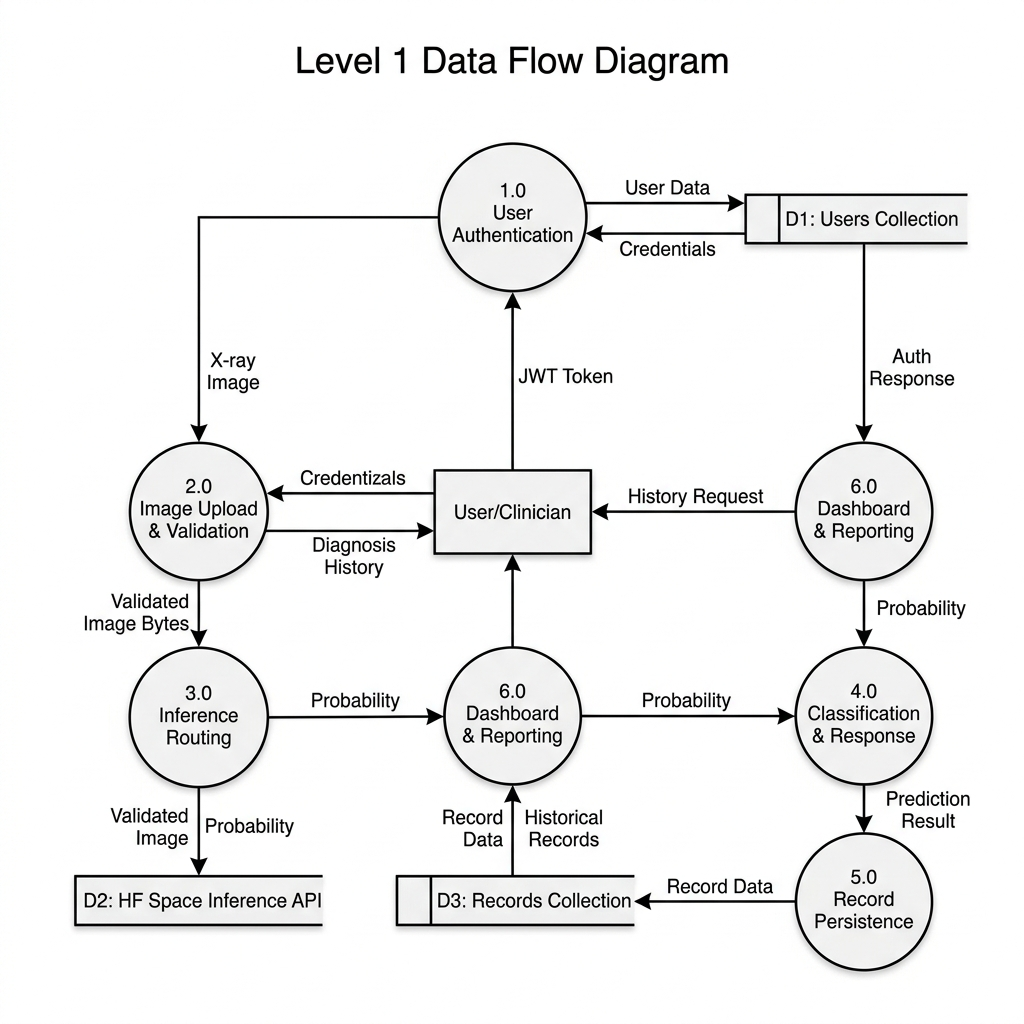
\includegraphics[width=0.95\textwidth]{dfd_level1.png}
\caption{Level 1 Data Flow Diagram}
\label{fig:dfd_level1}
\end{figure}

\section{UML Diagrams}
\label{sec:uml}

\subsection{Use Case Diagram}

The primary actors and their interactions with the system are:

\begin{figure}[H]
\centering
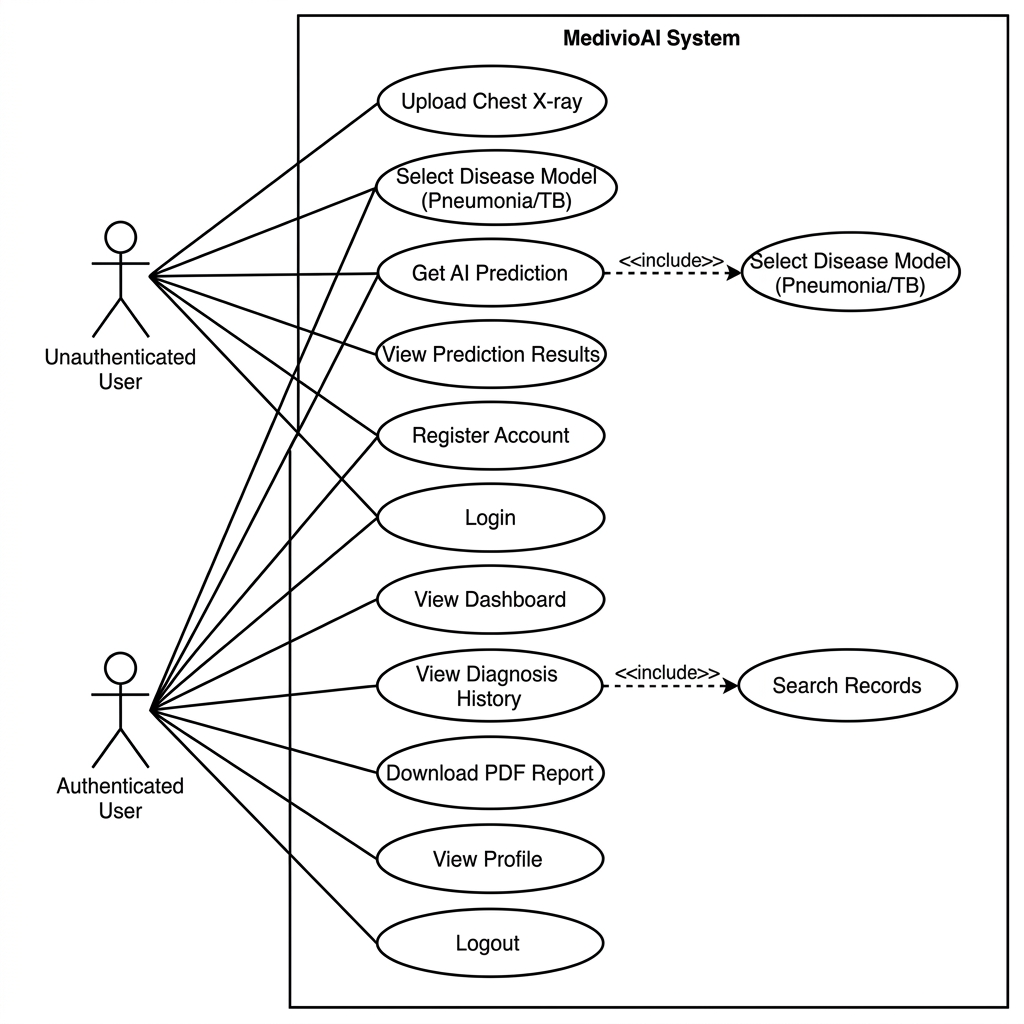
\includegraphics[width=0.85\textwidth]{use_case_diagram.png}
\caption{Use Case Diagram for MedivioAI}
\label{fig:usecase}
\end{figure}

\subsection{Sequence Diagram: Prediction Workflow}

The sequence diagram in Fig.~\ref{fig:sequence_predict} traces the end-to-end flow of a prediction request:

\begin{figure}[H]
\centering
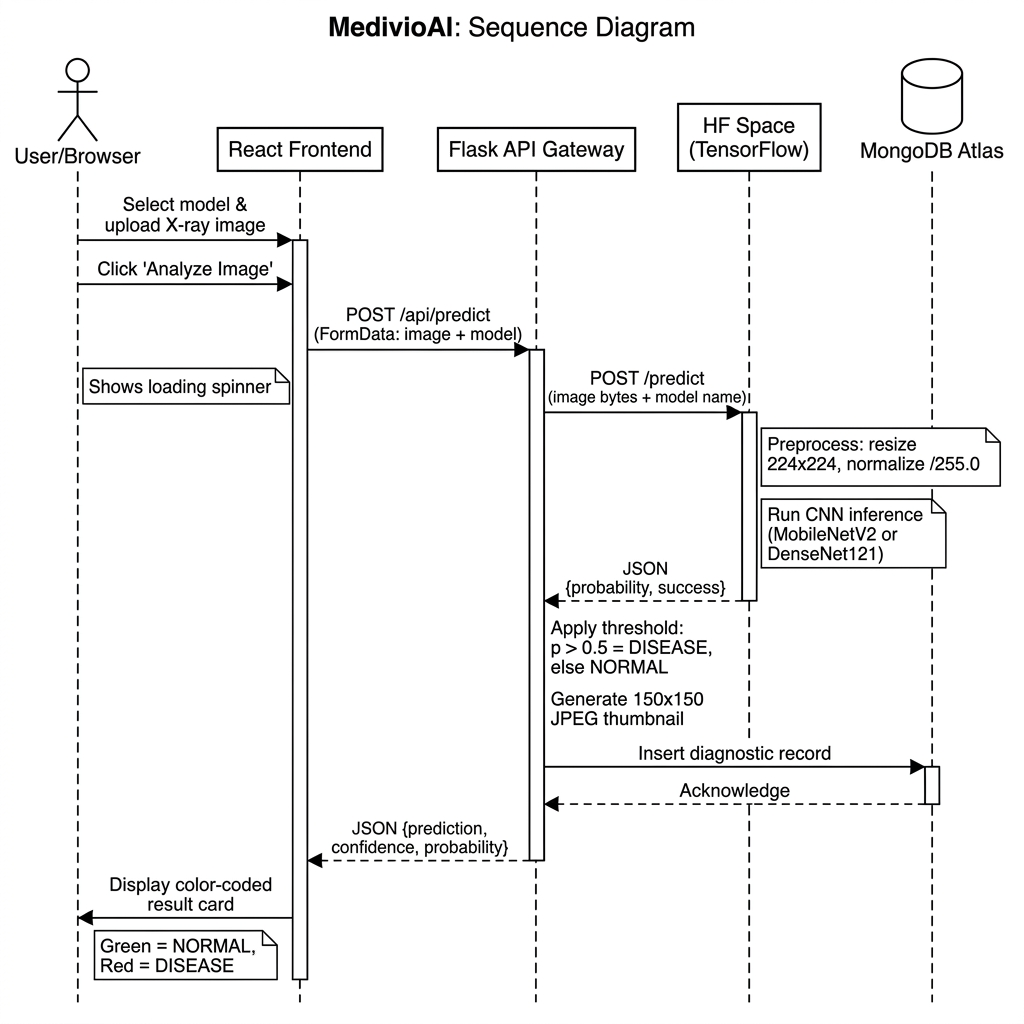
\includegraphics[width=0.95\textwidth]{sequence_diagram.png}
\caption{Sequence Diagram for the Prediction Workflow}
\label{fig:sequence_predict}
\end{figure}

\subsection{Component Diagram}

\begin{figure}[H]
\centering
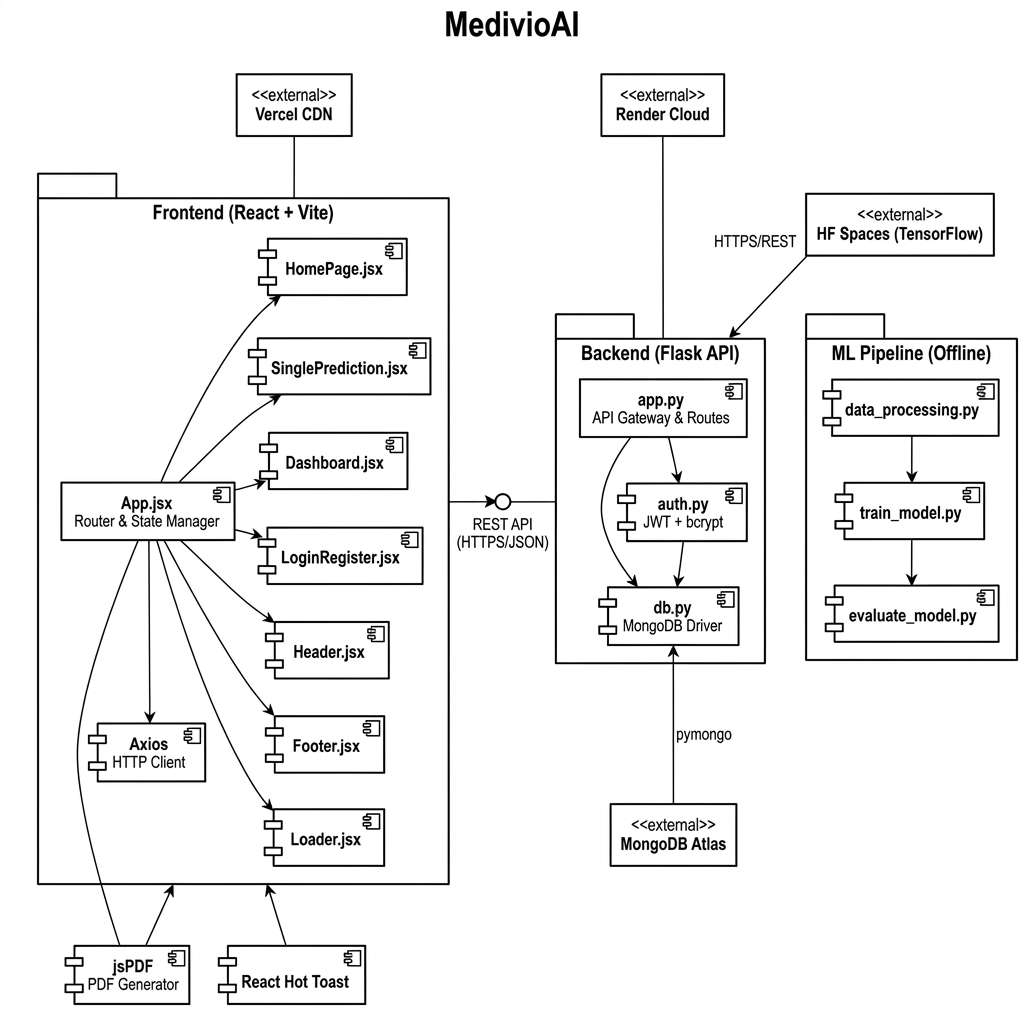
\includegraphics[width=0.95\textwidth]{component_diagram.png}
\caption{Component Diagram showing package dependencies}
\label{fig:component}
\end{figure}

\section{Entity-Relationship Diagram}
\label{sec:er_diagram}

Although MongoDB is a document-oriented (NoSQL) database and does not enforce a rigid schema, the application's data model can be represented as a logical ER diagram to clarify the relationships between entities.

\begin{figure}[H]
\centering
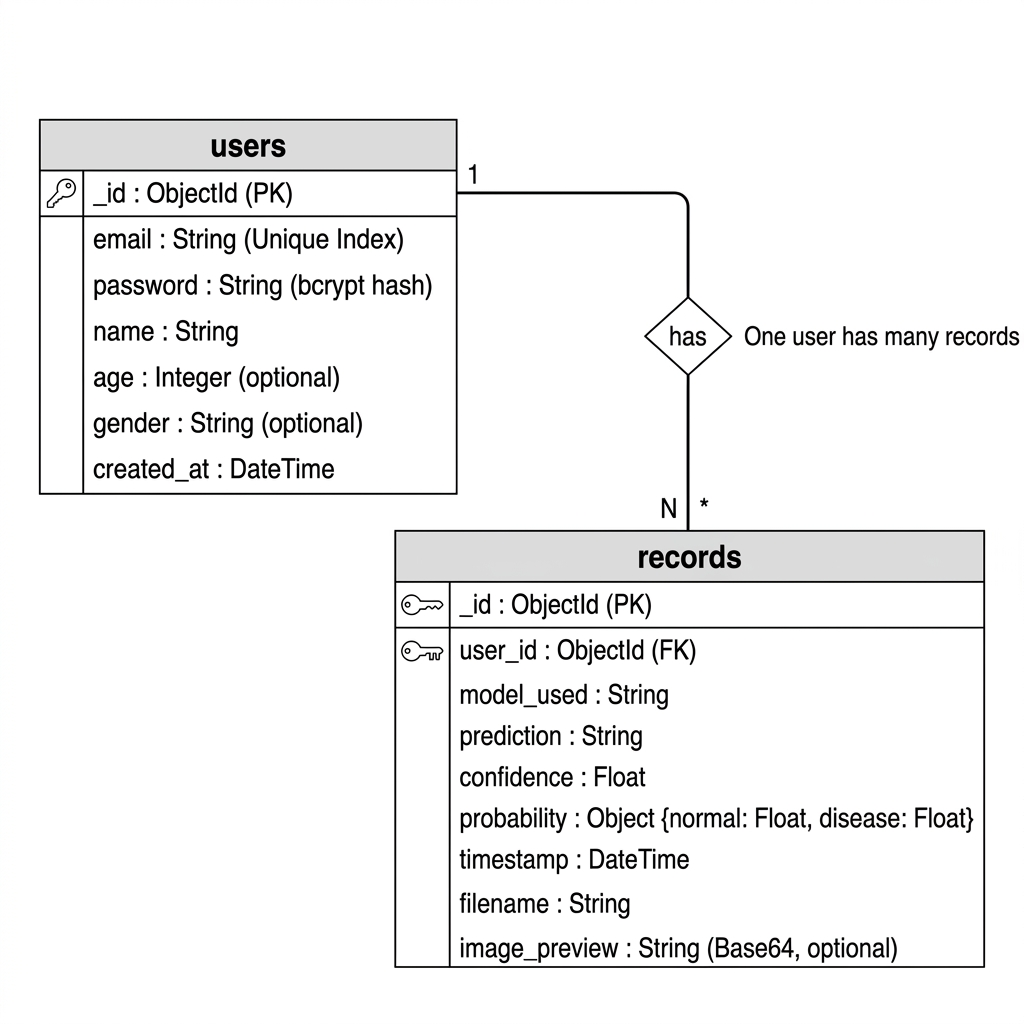
\includegraphics[width=0.85\textwidth]{er_diagram.png}
\caption{Logical Entity-Relationship Diagram}
\label{fig:er_diagram}
\end{figure}

\section{CNN Model Architecture}
\label{sec:cnn_architecture}

\subsection{Pneumonia Detection Model (MobileNetV2)}
\label{subsec:pneumonia_arch}

The Pneumonia detection model is constructed as a Keras Sequential model with the following layers:

\begin{table}[H]
\centering
\caption{Pneumonia detection model architecture (MobileNetV2-based)}
\label{tab:pneumonia_arch}
\begin{tabular}{llr}
\toprule
\textbf{Layer} & \textbf{Description} & \textbf{Output Shape} \\
\midrule
Input & RGB image & $(224, 224, 3)$ \\
MobileNetV2 & ImageNet-pretrained, \texttt{include\_top=False} & $(7, 7, 1280)$ \\
GlobalAveragePooling2D & Spatial averaging & $(1280)$ \\
Dense (128, ReLU) & Fully connected & $(128)$ \\
Dropout (0.5) & Regularisation & $(128)$ \\
Dense (1, Sigmoid) & Binary classifier & $(1)$ \\
\bottomrule
\end{tabular}
\end{table}

\subsection{Tuberculosis Detection Model (DenseNet121)}
\label{subsec:tb_arch}

The Tuberculosis detection model uses DenseNet121 as the feature extractor with additional regularisation layers:

\begin{table}[H]
\centering
\caption{Tuberculosis detection model architecture (DenseNet121-based)}
\label{tab:tb_arch}
\begin{tabular}{llr}
\toprule
\textbf{Layer} & \textbf{Description} & \textbf{Output Shape} \\
\midrule
Input & RGB image & $(224, 224, 3)$ \\
DenseNet121 & ImageNet-pretrained, \texttt{include\_top=False} & $(7, 7, 1024)$ \\
GlobalAveragePooling2D & Spatial averaging & $(1024)$ \\
BatchNormalization & Normalise activations & $(1024)$ \\
Dropout (0.5) & Regularisation & $(1024)$ \\
Dense (256, ReLU) & Fully connected & $(256)$ \\
BatchNormalization & Normalise activations & $(256)$ \\
Dropout (0.3) & Regularisation & $(256)$ \\
Dense (1, Sigmoid) & Binary classifier & $(1)$ \\
\bottomrule
\end{tabular}
\end{table}

\subsection{Training Hyperparameters}

\begin{table}[H]
\centering
\caption{Training hyperparameters for both models}
\label{tab:hyperparams}
\begin{tabular}{lcc}
\toprule
\textbf{Parameter} & \textbf{Pneumonia Model} & \textbf{TB Model} \\
\midrule
Input Resolution & $224 \times 224$ & $224 \times 224$ \\
Batch Size & 32 & 32 \\
Total Epochs & 50 & 50 + 20 (fine-tune) \\
Phase 1 LR & $1 \times 10^{-4}$ & $1 \times 10^{-4}$ \\
Phase 2 LR & $1 \times 10^{-5}$ & $1 \times 10^{-5}$ \\
Loss Function & Binary Cross-Entropy & Binary Cross-Entropy \\
Optimiser & Adam & Adam \\
Early Stopping Patience & 10 epochs & 10 epochs \\
LR Reduction Factor & 0.5 & 0.5 \\
Frozen Layers (Phase 1) & All base layers & All base layers \\
Unfrozen Layers (Phase 2) & Last 54 layers & Last 50 layers \\
\bottomrule
\end{tabular}
\end{table}

% ============================================================================
% CHAPTER 5: SOFTWARE AND HARDWARE REQUIREMENTS
% ============================================================================
\chapter{Software and Hardware Requirements}
\label{chap:requirements}

\section{Software Requirements}
\label{sec:software_req}

\subsection{Frontend Technologies}

\begin{table}[H]
\centering
\caption{Frontend software dependencies}
\label{tab:frontend_deps}
\begin{tabular}{llp{7cm}}
\toprule
\textbf{Technology} & \textbf{Version} & \textbf{Purpose} \\
\midrule
React & 19.1.1 & Component-based UI library \\
Vite (Rolldown) & 7.1.14 & Build tool and development server \\
TailwindCSS & 4.1.17 & Utility-first CSS framework \\
Axios & 1.13.2 & HTTP client for API requests \\
jsPDF & 4.2.1 & Client-side PDF generation \\
Lucide React & 0.553.0 & Icon library \\
React Hot Toast & 2.6.0 & Toast notification system \\
Styled Components & 6.4.3 & CSS-in-JS for the Loader component \\
Node.js & $\geq$ 18.x & JavaScript runtime environment \\
\bottomrule
\end{tabular}
\end{table}

\subsection{Backend Technologies}

\begin{table}[H]
\centering
\caption{Backend software dependencies}
\label{tab:backend_deps}
\begin{tabular}{llp{7cm}}
\toprule
\textbf{Technology} & \textbf{Version} & \textbf{Purpose} \\
\midrule
Python & 3.9 / 3.10 & Programming language \\
Flask & 3.0.0 & Lightweight WSGI web framework \\
Flask-CORS & 4.0.0 & Cross-Origin Resource Sharing \\
PyMongo & 4.10.1 & MongoDB driver for Python \\
PyJWT & 2.8.0 & JSON Web Token encoding/decoding \\
bcrypt & 4.1.2 & Password hashing library \\
Pillow & 12.0.0 & Image processing (thumbnails) \\
Requests & 2.32.5 & HTTP client for HF Space calls \\
python-dotenv & 1.0.1 & Environment variable management \\
Gunicorn & latest & Production WSGI HTTP server \\
dnspython & 2.6.1 & DNS toolkit for MongoDB SRV URIs \\
\bottomrule
\end{tabular}
\end{table}

\subsection{Machine Learning and Model Training}

\begin{table}[H]
\centering
\caption{ML/DL software dependencies}
\label{tab:ml_deps}
\begin{tabular}{llp{7cm}}
\toprule
\textbf{Technology} & \textbf{Version} & \textbf{Purpose} \\
\midrule
TensorFlow & 2.16.1 & Deep learning framework \\
Keras & 3.1.1 & High-level neural network API \\
NumPy & latest & Numerical computing \\
Matplotlib & latest & Training history visualisation \\
scikit-learn & latest & Evaluation metrics (confusion matrix, classification report) \\
Seaborn & latest & Statistical data visualisation \\
\bottomrule
\end{tabular}
\end{table}

\subsection{Cloud Services and Deployment}

\begin{table}[H]
\centering
\caption{Cloud services used for deployment}
\label{tab:cloud_services}
\begin{tabular}{lp{4cm}p{6cm}}
\toprule
\textbf{Service} & \textbf{Tier} & \textbf{Purpose} \\
\midrule
Vercel & Free (Hobby) & Frontend hosting with global CDN \\
Render & Free & Backend Flask API hosting \\
Hugging Face Spaces & Free (Docker SDK) & Model inference container (16\,GB RAM) \\
MongoDB Atlas & Free (M0 Shared) & Cloud-hosted NoSQL database \\
\bottomrule
\end{tabular}
\end{table}

\section{Hardware Requirements}
\label{sec:hardware_req}

\subsection{Development Environment}

\begin{table}[H]
\centering
\caption{Minimum hardware requirements for development}
\label{tab:hw_dev}
\begin{tabular}{lp{8cm}}
\toprule
\textbf{Component} & \textbf{Specification} \\
\midrule
Processor & Intel Core i5 (8th Gen) or equivalent / Apple M1 \\
RAM & 8 GB (16 GB recommended for model training) \\
Storage & 10 GB free disk space (SSD recommended) \\
GPU & NVIDIA GPU with CUDA support (optional; recommended for training) \\
Operating System & Windows 10/11, macOS 12+, or Ubuntu 20.04+ \\
Network & Stable internet connection (for MongoDB Atlas and API calls) \\
\bottomrule
\end{tabular}
\end{table}

\subsection{Production Environment}

In the deployed production configuration, all computation is performed on cloud infrastructure. The end user requires only a modern web browser (Chrome 90+, Firefox 88+, Safari 14+, Edge 90+) and an internet connection. No local software installation is needed.

% ============================================================================
% CHAPTER 6: CODE TEMPLATES
% ============================================================================
\chapter{Code Templates}
\label{chap:code}

This chapter describes the code architecture of the MedivioAI platform, explaining each module's classes, functions, input parameters, output values, and database schema.

\section{Backend Modules}
\label{sec:backend_modules}

\subsection{Module: \texttt{app.py} --- Flask Application Entry Point}
\label{subsec:app_py}

The \texttt{app.py} file serves as the central API gateway, defining all REST endpoints. Table~\ref{tab:app_endpoints} summarises the six API endpoints exposed by the application.

\begin{table}[H]
\centering
\caption{REST API endpoints defined in \texttt{app.py}}
\label{tab:app_endpoints}
\begin{tabularx}{\textwidth}{lllX}
\toprule
\textbf{Method} & \textbf{Endpoint} & \textbf{Access} & \textbf{Description} \\
\midrule
GET & \texttt{/api/health} & Public & Returns server status and inference URL \\
POST & \texttt{/api/auth/register} & Public & Creates a new user account \\
POST & \texttt{/api/auth/login} & Public & Authenticates user, returns JWT \\
GET & \texttt{/api/auth/profile} & Auth & Returns authenticated user's profile \\
GET & \texttt{/api/records} & Auth & Retrieves user's diagnostic history \\
POST & \texttt{/api/predict} & Public/Auth & Accepts image, returns prediction \\
\bottomrule
\end{tabularx}
\end{table}

\textbf{Key Function: \texttt{predict()}}

\begin{itemize}
    \item \textbf{Input Parameters:} Multipart form data containing an image file (key: \texttt{image}) and a model selector string (key: \texttt{model}, values: \texttt{``pneumonia''} or \texttt{``tuberculosis''}).
    \item \textbf{Processing:}
    \begin{enumerate}
        \item Reads raw bytes from the uploaded file.
        \item Forwards the bytes to the Hugging Face Space endpoint (\texttt{HF\_SPACE\_URL}) via \texttt{requests.post()}.
        \item Parses the JSON response to extract the probability value.
        \item Applies the 0.5 threshold to determine the predicted class.
        \item If an \texttt{Authorization} header is present, optionally decodes the JWT to identify the user and persists a diagnostic record (including a 150$\times$150 JPEG thumbnail) to the \texttt{records} collection.
    \end{enumerate}
    \item \textbf{Output:} JSON object containing \texttt{success} (boolean), \texttt{model\_used} (string), \texttt{prediction} (string), \texttt{confidence} (float), and \texttt{probability} (object with class-wise percentages).
\end{itemize}

\subsection{Module: \texttt{auth.py} --- Authentication Utilities}
\label{subsec:auth_py}

This module provides four core authentication functions:

\begin{table}[H]
\centering
\caption{Functions in \texttt{auth.py}}
\label{tab:auth_functions}
\begin{tabularx}{\textwidth}{lp{3.5cm}p{3cm}X}
\toprule
\textbf{Function} & \textbf{Input} & \textbf{Output} & \textbf{Description} \\
\midrule
\texttt{hash\_password()} & \texttt{password}: str & \texttt{str} (hash) & Generates a bcrypt salt and returns the hashed password string \\
\texttt{check\_password()} & \texttt{password}: str, \texttt{hashed}: str & \texttt{bool} & Compares plaintext password against stored bcrypt hash \\
\texttt{generate\_token()} & \texttt{user\_id}: ObjectId, \texttt{expires\_in\_days}: int & \texttt{str} (JWT) & Encodes a JWT with \texttt{sub}, \texttt{exp}, and \texttt{iat} claims using HS256 \\
\texttt{@token\_required} & (decorator) & (decorated fn) & Extracts and validates JWT from the \texttt{Authorization} header; populates \texttt{g.current\_user} \\
\bottomrule
\end{tabularx}
\end{table}

\subsection{Module: \texttt{db.py} --- Database Connection Manager}
\label{subsec:db_py}

The \texttt{db.py} module initialises the MongoDB connection and exports two collection handles: \texttt{users\_collection} and \texttt{records\_collection}. A notable design decision is the inclusion of an \textbf{in-memory fallback}: if the MongoDB connection fails (e.g., due to network issues or missing credentials), the module instantiates \texttt{InMemoryCollection} objects that implement the same interface (\texttt{find\_one()}, \texttt{insert\_one()}, \texttt{find()}) using Python lists and deep copies. This enables local development and testing without a live database.

The \texttt{InMemoryCursor} class implements the \texttt{sort()} method to replicate MongoDB's sort behaviour, and the \texttt{InMemoryInsertResult} class wraps the inserted ObjectId for API compatibility.

\section{Database Schema}
\label{sec:db_schema}

\subsection{Collection: \texttt{users}}

\begin{table}[H]
\centering
\caption{Schema for the \texttt{users} collection}
\label{tab:users_schema}
\begin{tabularx}{\textwidth}{llcX}
\toprule
\textbf{Field} & \textbf{Data Type} & \textbf{Required} & \textbf{Description} \\
\midrule
\texttt{\_id} & ObjectId & Auto & MongoDB primary key \\
\texttt{email} & String & Yes & User email (unique index) \\
\texttt{password} & String & Yes & bcrypt-hashed password \\
\texttt{name} & String & Yes & User's full name \\
\texttt{age} & Integer & No & User's age \\
\texttt{gender} & String & No & Gender (Male / Female / Other) \\
\texttt{created\_at} & DateTime & Auto & UTC timestamp of registration \\
\bottomrule
\end{tabularx}
\end{table}

\subsection{Collection: \texttt{records}}

\begin{table}[H]
\centering
\caption{Schema for the \texttt{records} collection}
\label{tab:records_schema}
\begin{tabularx}{\textwidth}{llcX}
\toprule
\textbf{Field} & \textbf{Data Type} & \textbf{Required} & \textbf{Description} \\
\midrule
\texttt{\_id} & ObjectId & Auto & MongoDB primary key \\
\texttt{user\_id} & ObjectId & Yes & Foreign key referencing \texttt{users.\_id} \\
\texttt{model\_used} & String & Yes & Model name (\texttt{pneumonia} / \texttt{tuberculosis}) \\
\texttt{prediction} & String & Yes & Classification label \\
\texttt{confidence} & Float & Yes & Confidence percentage (0--100) \\
\texttt{probability} & Object & Yes & \{normal: float, [disease]: float\} \\
\texttt{timestamp} & DateTime & Yes & UTC timestamp of prediction \\
\texttt{filename} & String & Yes & Original uploaded filename \\
\texttt{image\_preview} & String & No & Base64-encoded JPEG thumbnail \\
\bottomrule
\end{tabularx}
\end{table}

\section{Frontend Components}
\label{sec:frontend_components}

\subsection{Component: \texttt{App.jsx} --- Application Root and Router}

The root component manages application-level state (current page, authentication token, user object) and implements a manual page router via a \texttt{switch} statement in \texttt{renderPage()}. It supports the following page identifiers: \texttt{home}, \texttt{auth}, \texttt{dashboard}, \texttt{single}, \texttt{scan-pneumonia}, and \texttt{scan-tb}.

\textbf{State persistence:} The JWT token is stored in \texttt{localStorage} for persistence across browser sessions. The current page identifier is stored in \texttt{sessionStorage} to survive page refreshes within a session. The user object is serialised to JSON in \texttt{localStorage}.

\subsection{Component: \texttt{SinglePrediction.jsx} --- Scan Interface}

\begin{itemize}
    \item \textbf{Props:} \texttt{mode} (string: \texttt{``pneumonia''} or \texttt{``tuberculosis''}), \texttt{token} (string or null), \texttt{onBack} (callback function).
    \item \textbf{State:} \texttt{selectedFile}, \texttt{preview} (base64 Data URL), \texttt{loading} (boolean), \texttt{result} (prediction JSON).
    \item \textbf{Key Methods:}
    \begin{itemize}
        \item \texttt{handleFileSelect(event)}: Validates MIME type, reads file as Data URL for preview.
        \item \texttt{handleDrop(event)}: Handles drag-and-drop file selection.
        \item \texttt{handleAnalyze()}: Constructs \texttt{FormData}, sends POST request to \texttt{/api/predict} with optional \texttt{Bearer} token.
        \item \texttt{handleDownloadReport()}: Generates a PDF report using jsPDF with metadata, prediction details, disclaimer, and embedded image preview.
        \item \texttt{handleReset()}: Clears all state to allow a new scan.
    \end{itemize}
\end{itemize}

\subsection{Component: \texttt{Dashboard.jsx} --- Patient Portal}

\begin{itemize}
    \item \textbf{Props:} \texttt{token} (string), \texttt{user} (object), \texttt{onNavigate} (callback).
    \item \textbf{State:} \texttt{records} (array), \texttt{loading} (boolean), \texttt{searchTerm} (string).
    \item \textbf{Key Methods:}
    \begin{itemize}
        \item \texttt{fetchRecords()}: Sends authenticated GET request to \texttt{/api/records} and populates the records state.
        \item \texttt{handleDownloadReport(record)}: Generates a PDF report from a historical record, including patient name, email, age, and gender.
        \item \texttt{filteredRecords}: Computed array that filters records by prediction, model, or filename based on the search term.
    \end{itemize}
\end{itemize}

\subsection{Component: \texttt{LoginRegister.jsx} --- Authentication Form}

A dual-purpose form component that toggles between Sign In and Create Account modes using a tab-based interface. On submission, it sends a POST request to \texttt{/api/auth/login} or \texttt{/api/auth/register} and calls the \texttt{onAuthSuccess} callback with the returned token and user object upon success.

\subsection{Component: \texttt{Header.jsx} --- Navigation Bar}

A responsive sticky header with desktop and mobile navigation. Navigation items are dynamically constructed: the \texttt{Dashboard} tab appears only when a user is authenticated. The component renders conditional login/logout buttons based on authentication state.

\subsection{Component: \texttt{Loader.jsx} --- Splash Screen}

A styled-components-based animated loader displayed for 5 seconds on initial application load. The animation consists of three bouncing circles with gradient fills and drop shadows, implemented using CSS keyframe animations.

\section{Model Training Scripts}
\label{sec:training_scripts}

\subsection{Pneumonia Model: \texttt{pneumonia/train\_model.py}}

\begin{itemize}
    \item \textbf{Data Augmentation (Training):} Rotation ($\pm$20°), width/height shift (20\%), horizontal flip, zoom (20\%), shear (20\%), pixel rescaling ($\div$255).
    \item \textbf{Phase 1 (Epochs 1--20):} All MobileNetV2 layers frozen. Learning rate: $10^{-4}$.
    \item \textbf{Phase 2 (Epochs 21--50):} First 100 MobileNetV2 layers remain frozen; remaining layers unfrozen. Learning rate: $10^{-5}$.
    \item \textbf{Callbacks:} ModelCheckpoint (best \texttt{val\_accuracy}), EarlyStopping (patience 10, restore best weights), ReduceLROnPlateau (factor 0.5, patience 5, min LR $10^{-7}$), CSVLogger.
    \item \textbf{Metrics Tracked:} Accuracy, Precision, Recall.
\end{itemize}

\subsection{Tuberculosis Model: \texttt{tuberculosis/train\_model.py}}

\begin{itemize}
    \item \textbf{Data Augmentation (Training):} Rotation ($\pm$20°), width/height shift (20\%), zoom (20\%), shear (15\%), horizontal flip, brightness range [0.8, 1.2], pixel rescaling ($\div$255).
    \item \textbf{Phase 1 (Epochs 1--50):} All DenseNet121 layers frozen. Learning rate: $10^{-4}$.
    \item \textbf{Phase 2 (Epochs 51--70):} Last 50 DenseNet121 layers unfrozen. Learning rate: $10^{-5}$.
    \item \textbf{Callbacks:} ModelCheckpoint (best \texttt{val\_accuracy}), EarlyStopping (patience 10), ReduceLROnPlateau, TensorBoard.
    \item \textbf{Metrics Tracked:} Accuracy, Precision, Recall, AUC.
    \item \textbf{Configuration:} Managed through a dedicated \texttt{Config} class with centralised hyperparameter definitions.
\end{itemize}

% ============================================================================
% CHAPTER 7: OUTPUT SCREENS / EXPERIMENTAL RESULTS
% ============================================================================
\chapter{Output Screens and Experimental Results}
\label{chap:results}

\section{User Interface Screens}
\label{sec:ui_screens}

This section presents the key user interface screens of the MedivioAI web application. All interfaces are fully responsive and employ a dark-themed design with glassmorphism effects, consistent with modern healthcare application aesthetics.

\subsection{Home Page}

The landing page (Fig.~\ref{fig:homepage}) features a hero section with a call-to-action button, a visual status card showing active disease models, and a four-column feature grid highlighting the platform's capabilities.

\begin{figure}[H]
\centering
\fbox{\parbox{0.85\textwidth}{\centering
\vspace{0.3cm}
\textbf{[Screenshot Placeholder: Home Page]}\\
\small Insert screenshot of the MedivioAI homepage showing the hero section, status card, and feature grid.
\vspace{0.3cm}
}}
\caption{MedivioAI Home Page}
\label{fig:homepage}
\end{figure}

\subsection{Scan Type Selection}

After navigating to the Scan page, users are presented with two options: Pneumonia Scan and Tuberculosis Scan (Fig.~\ref{fig:scan_select}). Each card provides a brief description of the disease model and a ``Continue'' button.

\begin{figure}[H]
\centering
\fbox{\parbox{0.85\textwidth}{\centering
\vspace{0.3cm}
\textbf{[Screenshot Placeholder: Scan Selection Page]}\\
\small Insert screenshot showing the two scan type cards.
\vspace{0.3cm}
}}
\caption{Scan Type Selection Interface}
\label{fig:scan_select}
\end{figure}

\subsection{Image Upload and Analysis}

The prediction interface (Fig.~\ref{fig:upload}) features a drag-and-drop upload zone on the left and a results panel on the right. The model indicator badge confirms the selected disease model.

\begin{figure}[H]
\centering
\fbox{\parbox{0.85\textwidth}{\centering
\vspace{0.3cm}
\textbf{[Screenshot Placeholder: Upload and Analysis Interface]}\\
\small Insert screenshot showing image preview, Analyze button, and loading spinner.
\vspace{0.3cm}
}}
\caption{Image Upload and Analysis Interface}
\label{fig:upload}
\end{figure}

\subsection{Prediction Results}

Upon successful analysis, the results panel displays a colour-coded prediction card: green for NORMAL (with a checkmark icon) and red for a positive disease finding (with an alert icon). A confidence progress bar and percentage are prominently displayed. A ``Download report'' button enables PDF export (Fig.~\ref{fig:results}).

\begin{figure}[H]
\centering
\fbox{\parbox{0.85\textwidth}{\centering
\vspace{0.3cm}
\textbf{[Screenshot Placeholder: Prediction Results]}\\
\small Insert screenshots showing both NORMAL and DISEASE prediction outcomes.
\vspace{0.3cm}
}}
\caption{Prediction Results Display}
\label{fig:results}
\end{figure}

\subsection{Login and Registration}

The authentication interface (Fig.~\ref{fig:auth}) uses a tabbed layout with ``Sign In'' and ``Create Account'' tabs. The registration form collects name, email, password, age, and gender.

\begin{figure}[H]
\centering
\fbox{\parbox{0.85\textwidth}{\centering
\vspace{0.3cm}
\textbf{[Screenshot Placeholder: Login/Register Interface]}\\
\small Insert screenshot showing both sign-in and registration form variants.
\vspace{0.3cm}
}}
\caption{Authentication Interface (Login and Registration)}
\label{fig:auth}
\end{figure}

\subsection{Patient Dashboard}

The dashboard (Fig.~\ref{fig:dashboard}) provides a personalised welcome banner, patient profile card (left column), and a diagnosis history table (right column) with image thumbnails, prediction badges, confidence bars, timestamps, and PDF download buttons.

\begin{figure}[H]
\centering
\fbox{\parbox{0.85\textwidth}{\centering
\vspace{0.3cm}
\textbf{[Screenshot Placeholder: Patient Dashboard]}\\
\small Insert screenshot of the dashboard with profile and records table.
\vspace{0.3cm}
}}
\caption{Patient Dashboard with Diagnosis History}
\label{fig:dashboard}
\end{figure}

\section{Experimental Results: Model Performance}
\label{sec:model_results}

\subsection{Tuberculosis Detection Model Evaluation}

The DenseNet121-based TB detection model was evaluated on a held-out test set of 630 chest X-ray images (525 Normal, 105 Tuberculosis). The evaluation results, obtained from the automated evaluation pipeline (\texttt{tuberculosis/evaluate\_model.py}), are presented below.

\subsubsection{Overall Performance Metrics}

\begin{table}[H]
\centering
\caption{TB detection model --- overall performance metrics on the test set}
\label{tab:tb_metrics}
\begin{tabular}{lr}
\toprule
\textbf{Metric} & \textbf{Value} \\
\midrule
Test Accuracy & 98.89\% \\
Test Precision & 98.04\% \\
Test Recall (Sensitivity) & 95.24\% \\
F1-Score & 96.62\% \\
AUC-ROC & 0.9985 \\
AUC-PR & 0.9929 \\
Matthews Correlation Coefficient (MCC) & 0.9597 \\
Test Loss & 0.0379 \\
\bottomrule
\end{tabular}
\end{table}

\subsubsection{Confusion Matrix}

\begin{table}[H]
\centering
\caption{Confusion matrix for the TB detection model (630 test samples)}
\label{tab:tb_confusion}
\begin{tabular}{lcc}
\toprule
& \textbf{Predicted Normal} & \textbf{Predicted TB} \\
\midrule
\textbf{Actual Normal} (525) & 523 (TN) & 2 (FP) \\
\textbf{Actual TB} (105) & 5 (FN) & 100 (TP) \\
\bottomrule
\end{tabular}
\end{table}

The confusion matrix reveals that the model correctly classified 523 out of 525 Normal samples (specificity = 99.62\%) and 100 out of 105 Tuberculosis samples (sensitivity = 95.24\%). Only 2 false positives and 5 false negatives were observed.

\subsubsection{Per-Class Classification Report}

\begin{table}[H]
\centering
\caption{Per-class classification report for the TB detection model}
\label{tab:tb_class_report}
\begin{tabular}{lcccc}
\toprule
\textbf{Class} & \textbf{Precision} & \textbf{Recall} & \textbf{F1-Score} & \textbf{Support} \\
\midrule
Normal & 0.9905 & 0.9962 & 0.9934 & 525 \\
Tuberculosis & 0.9804 & 0.9524 & 0.9662 & 105 \\
\midrule
\textbf{Weighted Avg} & \textbf{0.9888} & \textbf{0.9889} & \textbf{0.9888} & \textbf{630} \\
\bottomrule
\end{tabular}
\end{table}

\subsubsection{ROC Curve}

\begin{figure}[H]
\centering
\fbox{\parbox{0.85\textwidth}{\centering
\vspace{0.3cm}
\textbf{[Plot Placeholder: ROC Curve]}\\
\small Insert the ROC curve plot from \texttt{evaluation\_results/tuberculosis/roc\_curve.png}.\\
AUC-ROC = 0.9985
\vspace{0.3cm}
}}
\caption{Receiver Operating Characteristic (ROC) curve for the TB detection model}
\label{fig:roc_curve}
\end{figure}

\subsubsection{Precision-Recall Curve}

\begin{figure}[H]
\centering
\fbox{\parbox{0.85\textwidth}{\centering
\vspace{0.3cm}
\textbf{[Plot Placeholder: Precision-Recall Curve]}\\
\small Insert the PR curve plot from \texttt{evaluation\_results/tuberculosis/precision\_recall\_curve.png}.\\
AUC-PR = 0.9929
\vspace{0.3cm}
}}
\caption{Precision-Recall curve for the TB detection model}
\label{fig:pr_curve}
\end{figure}

\subsection{Data Augmentation Strategy}

Both models employ runtime data augmentation during training to improve generalisation. The augmentation parameters are listed in Table~\ref{tab:augmentation}.

\begin{table}[H]
\centering
\caption{Data augmentation parameters applied during training}
\label{tab:augmentation}
\begin{tabular}{lcc}
\toprule
\textbf{Augmentation} & \textbf{Pneumonia Model} & \textbf{TB Model} \\
\midrule
Rotation Range & $\pm$20° & $\pm$20° \\
Width Shift & 20\% & 20\% \\
Height Shift & 20\% & 20\% \\
Horizontal Flip & Yes & Yes \\
Zoom Range & 20\% & 20\% \\
Shear Range & 20\% & 15\% \\
Brightness Range & --- & [0.8, 1.2] \\
Fill Mode & Nearest & Nearest \\
Pixel Rescaling & $\div$255 & $\div$255 \\
\bottomrule
\end{tabular}
\end{table}

\subsection{Analysis of Results}

The TB detection model's performance metrics indicate strong discriminative capability across both classes. An AUC-ROC of 0.9985 demonstrates near-perfect separability between Normal and Tuberculosis classes. The slightly lower recall for the Tuberculosis class (95.24\% vs. 99.62\% for Normal) is expected given the class imbalance in the test set (525 Normal vs. 105 TB) and the higher clinical bar for detecting subtle TB manifestations in radiographs.

The 5 false negatives represent cases where genuine TB patterns were not detected. In a clinical deployment, this would translate to a small percentage of TB cases being missed, which underscores the importance of using this system as a screening aid rather than a standalone diagnostic tool. The 2 false positives (Normal cases flagged as TB) would result in unnecessary follow-up investigations, which, while undesirable, carry a lower clinical risk than missed diagnoses.

% ============================================================================
% CHAPTER 8: CONCLUSIONS
% ============================================================================
\chapter{Conclusions}
\label{chap:conclusions}

\section{Summary of Work}
\label{sec:summary}

This project successfully designed, implemented, and deployed \textbf{MedivioAI}, a full-stack AI-powered web application for the early detection and screening of Pneumonia and Tuberculosis from Chest X-ray images. The key contributions of this work are summarised as follows:

\begin{enumerate}[label=\arabic*.]
    \item \textbf{Dual-Disease CNN Models:} Two dedicated binary classifiers were trained using transfer learning: a MobileNetV2-based model for Pneumonia detection and a DenseNet121-based model for Tuberculosis detection. Both models employed a two-phase training strategy (frozen base followed by selective fine-tuning) with comprehensive data augmentation. The TB model achieved a test accuracy of 98.89\% and an AUC-ROC of 0.9985.

    \item \textbf{Three-Tier Microservice Architecture:} The platform was architected as a decoupled microservice system separating the React frontend (Vercel), Flask API gateway (Render), and TensorFlow inference container (Hugging Face Spaces). This design overcame the 512\,MB RAM constraint of free-tier hosting by offloading compute-intensive inference to a 16\,GB container.

    \item \textbf{Secure Authentication and Data Persistence:} JWT-based authentication with bcrypt password hashing was implemented to protect user accounts. MongoDB Atlas provides cloud-based persistence for user profiles and diagnostic records, including base64-encoded X-ray thumbnails.

    \item \textbf{Responsive User Interface:} A modern, responsive single-page application built with React 19 and TailwindCSS provides an intuitive clinical workflow---from image upload through analysis to PDF report generation---with sub-3-second end-to-end latency.

    \item \textbf{Zero-Cost Deployment:} The entire platform operates exclusively on free-tier cloud services, demonstrating that production-quality medical AI tools can be deployed without hardware procurement or recurring infrastructure costs.
\end{enumerate}

\section{Limitations}
\label{sec:limitations}

The current implementation has the following limitations:

\begin{itemize}
    \item \textbf{Binary Classification Only:} Each model performs single-disease binary classification. Multi-label classification (detecting multiple concurrent conditions) is not supported.
    \item \textbf{No Interpretability:} The system does not provide visual explanations (e.g., Grad-CAM heatmaps) of which image regions influenced the prediction, limiting the clinician's ability to validate AI reasoning.
    \item \textbf{Free-Tier Constraints:} Render's free-tier instances spin down after periods of inactivity, introducing cold-start delays of 30--60 seconds for the first request.
    \item \textbf{Image Format Dependency:} The system is optimised for standard posteroanterior (PA) Chest X-ray images. Performance on lateral views, CT scans, or non-standard image formats has not been validated.
    \item \textbf{No DICOM Support:} Native medical imaging formats (DICOM) are not supported; images must be uploaded as JPEG or PNG.
\end{itemize}

\section{Future Enhancements}
\label{sec:future_work}

Based on the identified limitations and emerging trends in medical AI, the following enhancements are proposed for future iterations:

\begin{enumerate}[label=\arabic*.]
    \item \textbf{Grad-CAM Integration:} Implementing Gradient-weighted Class Activation Mapping to generate heatmap overlays on the X-ray image, highlighting the lung regions that most influenced the model's prediction. This would significantly improve clinical interpretability and trust.

    \item \textbf{Multi-Label Classification:} Extending the pipeline to screen for multiple respiratory conditions simultaneously (e.g., COVID-19, Atelectasis, Cardiomegaly, Pleural Effusion) using a multi-label classifier.

    \item \textbf{DICOM File Support:} Adding support for the Digital Imaging and Communications in Medicine (DICOM) standard to directly ingest medical-native \texttt{.dcm} image assets from radiology workstations.

    \item \textbf{PDF Report Enhancement:} Generating formal, institution-branded diagnostic reports with integrated Grad-CAM visualisations, patient metadata, and QR codes for verification.

    \item \textbf{Federated Learning:} Exploring federated learning approaches that allow model improvement from distributed hospital datasets without centralising sensitive patient data.
\end{enumerate}

\section{Concluding Remarks}
\label{sec:concluding}

MedivioAI demonstrates that the convergence of modern deep learning architectures, cloud-native microservice design, and open-source web technologies can produce a clinically relevant screening tool that is accessible, cost-effective, and technically rigorous. While the system is positioned as an experimental screening aid and not a certified medical device, the achieved performance metrics and architectural decisions provide a solid foundation for future development towards clinical deployment.

% ============================================================================
% REFERENCES
% ============================================================================
\newpage
\addcontentsline{toc}{chapter}{References}
\begin{thebibliography}{99}

\bibitem{krizhevsky2012}
A. Krizhevsky, I. Sutskever, and G. E. Hinton, `ImageNet Classification with Deep Convolutional Neural Networks', in \textit{Advances in Neural Information Processing Systems (NeurIPS)}, vol. 25, pp. 1097--1105, 2012.

\bibitem{simonyan2014}
K. Simonyan and A. Zisserman, `Very Deep Convolutional Networks for Large-Scale Image Recognition', in \textit{Proceedings of the International Conference on Learning Representations (ICLR)}, 2015.

\bibitem{szegedy2015}
C. Szegedy, W. Liu, Y. Jia, P. Sermanet, S. Reed, D. Anguelov, D. Erhan, V. Vanhoucke, and A. Rabinovich, `Going Deeper with Convolutions', in \textit{Proceedings of the IEEE Conference on Computer Vision and Pattern Recognition (CVPR)}, pp. 1--9, 2015.

\bibitem{he2016}
K. He, X. Zhang, S. Ren, and J. Sun, `Deep Residual Learning for Image Recognition', in \textit{Proceedings of the IEEE Conference on Computer Vision and Pattern Recognition (CVPR)}, pp. 770--778, 2016.

\bibitem{huang2017}
G. Huang, Z. Liu, L. van der Maaten, and K. Q. Weinberger, `Densely Connected Convolutional Networks', in \textit{Proceedings of the IEEE Conference on Computer Vision and Pattern Recognition (CVPR)}, pp. 4700--4708, 2017.

\bibitem{sandler2018}
M. Sandler, A. Howard, M. Zhu, A. Zhmoginov, and L.-C. Chen, `MobileNetV2: Inverted Residuals and Linear Bottlenecks', in \textit{Proceedings of the IEEE Conference on Computer Vision and Pattern Recognition (CVPR)}, pp. 4510--4520, 2018.

\bibitem{rajpurkar2017}
P. Rajpurkar, J. Irvin, K. Zhu, B. Yang, H. Mehta, T. Duan, D. Ding, A. Bagul, C. Langlotz, K. Shpanskaya, M. P. Lungren, and A. Y. Ng, `CheXNet: Radiologist-Level Pneumonia Detection on Chest X-Rays with Deep Learning', \textit{arXiv preprint arXiv:1711.05225}, 2017.

\bibitem{yosinski2014}
J. Yosinski, J. Clune, Y. Bengio, and H. Lipson, `How Transferable Are Features in Deep Neural Networks?', in \textit{Advances in Neural Information Processing Systems (NeurIPS)}, vol. 27, pp. 3320--3328, 2014.

\bibitem{shin2016}
H.-C. Shin, H. R. Roth, M. Gao, L. Lu, Z. Xu, I. Nogues, J. Yao, D. Mollura, and R. M. Summers, `Deep Convolutional Neural Networks for Computer-Aided Detection: CNN Architectures, Dataset Characteristics and Transfer Learning', \textit{IEEE Transactions on Medical Imaging}, vol. 35, no. 5, pp. 1285--1298, 2016.

\bibitem{pan2010}
S. J. Pan and Q. Yang, `A Survey on Transfer Learning', \textit{IEEE Transactions on Knowledge and Data Engineering}, vol. 22, no. 10, pp. 1345--1359, 2010.

\bibitem{kermany2018}
D. S. Kermany, M. Goldbaum, W. Cai, C. C. S. Valentim, H. Liang, S. L. Baxter, A. McKeown, G. Yang, X. Wu, F. Yan, J. Dong, M. K. Prasadha, J. Pei, M. Ting, J. Zhu, C. Li, S. Hewett, J. Dong, I. Ziyar, A. Shi, R. Zhang, L. Zheng, R. Hou, W. Shi, X. Fu, Y. Duan, V. A. N. Huu, C. Wen, E. D. Zhang, C. L. Zhang, O. Li, X. Wang, M. A. Singer, X. Sun, J. Xu, A. Tafreshi, M. A. Lewis, H. Xia, and K. Zhang, `Identifying Medical Diagnoses and Treatable Diseases by Image-Based Deep Learning', \textit{Cell}, vol. 172, no. 5, pp. 1122--1131, 2018.

\bibitem{stephen2019}
O. Stephen, M. Sain, U. J. Maduh, and D.-U. Jeong, `An Efficient Deep Learning Approach to Pneumonia Classification in Healthcare', \textit{Journal of Healthcare Engineering}, vol. 2019, Article ID 4180949, 2019.

\bibitem{lakhani2017}
P. Lakhani and B. Sundaram, `Deep Learning at Chest Radiography: Automated Classification of Pulmonary Tuberculosis by Using Convolutional Neural Networks', \textit{Radiology}, vol. 284, no. 2, pp. 574--582, 2017.

\bibitem{hwang2016}
S. Hwang, H.-E. Kim, J. Jeong, and H.-J. Kim, `A Novel Approach for Tuberculosis Screening Based on Deep Convolutional Neural Networks', in \textit{Proceedings of SPIE Medical Imaging}, vol. 9785, pp. 97852W, 2016.

\bibitem{qureai}
Qure.ai, `qXR --- AI Powered Chest X-Ray Interpretation', Available: https://qure.ai/product/qxr/, 2023.

\bibitem{lunit}
Lunit Inc., `INSIGHT CXR --- AI Solution for Chest X-Ray Analysis', Available: https://www.lunit.io/en/products/insight-cxr, 2023.

\bibitem{chexpert}
J. Irvin, P. Rajpurkar, M. Ko, Y. Yu, S. Ciurea-Ilcus, C. Chute, H. Marklund, B. Haghgoo, R. Ball, K. Shpanskaya, J. Seekins, D. A. Mong, S. S. Halabi, J. K. Sandberg, R. Jones, D. B. Larson, C. P. Langlotz, B. N. Patel, M. P. Lungren, and A. Y. Ng, `CheXpert: A Large Chest Radiograph Dataset with Uncertainty Labels and Expert Comparison', in \textit{Proceedings of the AAAI Conference on Artificial Intelligence}, vol. 33, pp. 590--597, 2019.

\end{thebibliography}

% ============================================================================
% APPENDIX
% ============================================================================
\appendix
\chapter{Project Directory Structure}
\label{app:structure}

\begin{lstlisting}[language={}, caption={Complete project directory structure}, label={lst:directory}]
MedivioAI/
|-- backend/
|   |-- app.py                   # Flask API Gateway (Entry Point)
|   |-- auth.py                  # JWT Authentication Utilities
|   |-- db.py                    # MongoDB Connection Manager
|   |-- requirements.txt         # Python Dependencies
|   |-- test_auth_db.py          # Backend Verification Script
|   |-- pneumonia/
|   |   |-- data_processing.py   # Dataset Analysis & Visualisation
|   |   |-- train_model.py       # MobileNetV2 Training Pipeline
|   |   |-- evaluate_model.py    # Pneumonia Model Evaluation
|   |   |-- plot_pneumonia_training.py
|   |-- tuberculosis/
|   |   |-- data_processing.py   # TB Dataset Processing & Splitting
|   |   |-- train_model.py       # DenseNet121 Training Pipeline
|   |   |-- evaluate_model.py    # TB Model Evaluation
|   |   |-- plot_tb_training.py
|   |-- validate_xray/
|   |   |-- train.py             # X-Ray Validator (EfficientNetB0)
|   |   |-- data_processing.py   # Validator Data Preparation
|   |   |-- evaluation.py        # Validator Evaluation
|   |-- models/                  # Saved Keras Model Files
|   |-- data/                    # Training Datasets
|   |-- evaluation_results/      # Evaluation Outputs (JSON, PNG)
|   |-- logs/                    # Training Logs (CSV, TensorBoard)
|-- frontend/
|   |-- index.html               # HTML Entry Point
|   |-- package.json             # Node.js Dependencies
|   |-- vite.config.js           # Vite Build Configuration
|   |-- vercel.json              # Vercel SPA Routing Config
|   |-- src/
|   |   |-- main.jsx             # React DOM Entry Point
|   |   |-- App.jsx              # Application Root & Router
|   |   |-- App.css              # Global Styles & Animations
|   |   |-- components/
|   |   |   |-- HomePage.jsx     # Landing Page
|   |   |   |-- SinglePrediction.jsx  # Scan & Analysis Interface
|   |   |   |-- Dashboard.jsx    # Patient Portal & History
|   |   |   |-- LoginRegister.jsx # Authentication Forms
|   |   |   |-- Header.jsx       # Navigation Bar
|   |   |   |-- Footer.jsx       # Footer Component
|   |   |   |-- Loader.jsx       # Animated Splash Screen
|   |   |-- assets/              # Static Images
|-- README.md                    # Project Documentation
|-- LICENSE                      # MIT License
\end{lstlisting}

\chapter{Environment Variables Configuration}
\label{app:env}

\section{Backend Environment Variables (\texttt{backend/.env})}

\begin{lstlisting}[language={}, caption={Backend environment configuration}]
MONGO_URI=mongodb+srv://<db_user>:<password>@cluster.mongodb.net/medivioai
JWT_SECRET=your_jwt_signature_secret_key
\end{lstlisting}

\section{Frontend Environment Variables (\texttt{frontend/.env})}

\begin{lstlisting}[language={}, caption={Frontend environment configuration}]
VITE_API_URL=https://your-backend-onrender.com
\end{lstlisting}

\end{document}
